\documentclass[a4paper]{article}
\usepackage{geometry}
\geometry{left=1.5cm, right=1.5cm, top=1.5cm, bottom=1.5cm}
\usepackage[utf8]{inputenc}

\usepackage{hyperref}

\usepackage{amsmath}
\usepackage{amsfonts}
\usepackage{amssymb}
\usepackage{amsthm}
\usepackage{bbm}
\usepackage{interval}
\intervalconfig{
soft open fences
}
\usepackage{mathabx}
\usepackage{listings}
\theoremstyle{definition}
\newtheorem{definition}{Definition}[section]
\newtheorem{example}{Example}[section]
\newtheorem{lemma}{Lemma}[section]
\newtheorem{theorem}{Theorem}[section]
\newtheorem{corollary}{Corollary}[section]
\newtheorem{remark}{Remark}[section]

\usepackage{graphicx}
\usepackage{float}
\usepackage{caption}

\setlength\parindent{0pt}

\title{Deep RL Assignment2}
\author{Mufei Li \href{mufei.li@nyu.edu}{mufei.li@nyu.edu}}
\begin{document}
\maketitle

\section*{4 Implement Policy Gradient}

\subsection*{4.2}

\subsubsection*{1}

As required by instructions, we perform $6$ experiments on OpenAI's Gym environment CartPole-v0 to get a feel for how different settings impact the performance of policy gradient methods and plot below their learning curves (average return at each iteration) averaged over $5$ runs using different random seeds. The setting of each experiment can be specified by its name:
\begin{itemize}
\item \textbf{sb}: small batch size, we use $1000$
\item \textbf{lb}: large batch size, we use $5000$
\item \textbf{rtg}: use reward to go
\item \textbf{no$\rule{0.15cm}{0.15mm}$rtg}: do not use reward to go
\item \textbf{na}: normalize advantages
\item \textbf{dna}: do not normalize advantages
\end{itemize}

Besides the differences we mention above, all experiments use the same following setting:
\begin{itemize}
\item \textbf{discount factor}: $1.0$ (no discount)
\item \textbf{number of random seeds}: $5$, particularly we use $\{1, 11, 21, 31, 41\}$
\item \textbf{number of iterations for each random seed}: $100$
\item \textbf{max path length}: $200$, which is enforced by OpenAI's design of max number of timesteps allowed in an episode for CartPole-v0
\item \textbf{learning rate}: $0.005$
\item \textbf{optimization}: Adam with its default settings in PyTorch
\item \textbf{policy architecture}: in the order of nn.Linear$(4, 32)$, nn.Tanh, nn.Linear$(32, 2)$, followed by a softmax operation
\end{itemize}

To run the experiments, use the following command line configurations:
\begin{lstlisting}[language=bash]
python train_pg.py CartPole-v0 -n 100 -b 1000 -e 5 -dna -l 1 -s 32
    --exp_name sb_no_rtg_dna
python train_pg.py CartPole-v0 -n 100 -b 1000 -e 5 -rtg -dna -l 1 -s 32
    --exp_name sb_rtg_dna
python train_pg.py CartPole-v0 -n 100 -b 1000 -e 5 -rtg -l 1 -s 32
    --exp_name sb_rtg_na
python train_pg.py CartPole-v0 -n 100 -b 5000 -e 5 -dna -l 1 -s 32
    --exp_name lb_no_rtg_dna
python train_pg.py CartPole-v0 -n 100 -b 5000 -e 5 -rtg -dna -l 1 -s 32
    --exp_name lb_rtg_dna
python train_pg.py CartPole-v0 -n 100 -b 5000 -e 5 -rtg -l 1 -s 32
    --exp_name lb_rtg_na
\end{lstlisting}

\begin{figure}[H]
\centering
\begin{minipage}{.47\textwidth}
  \centering
  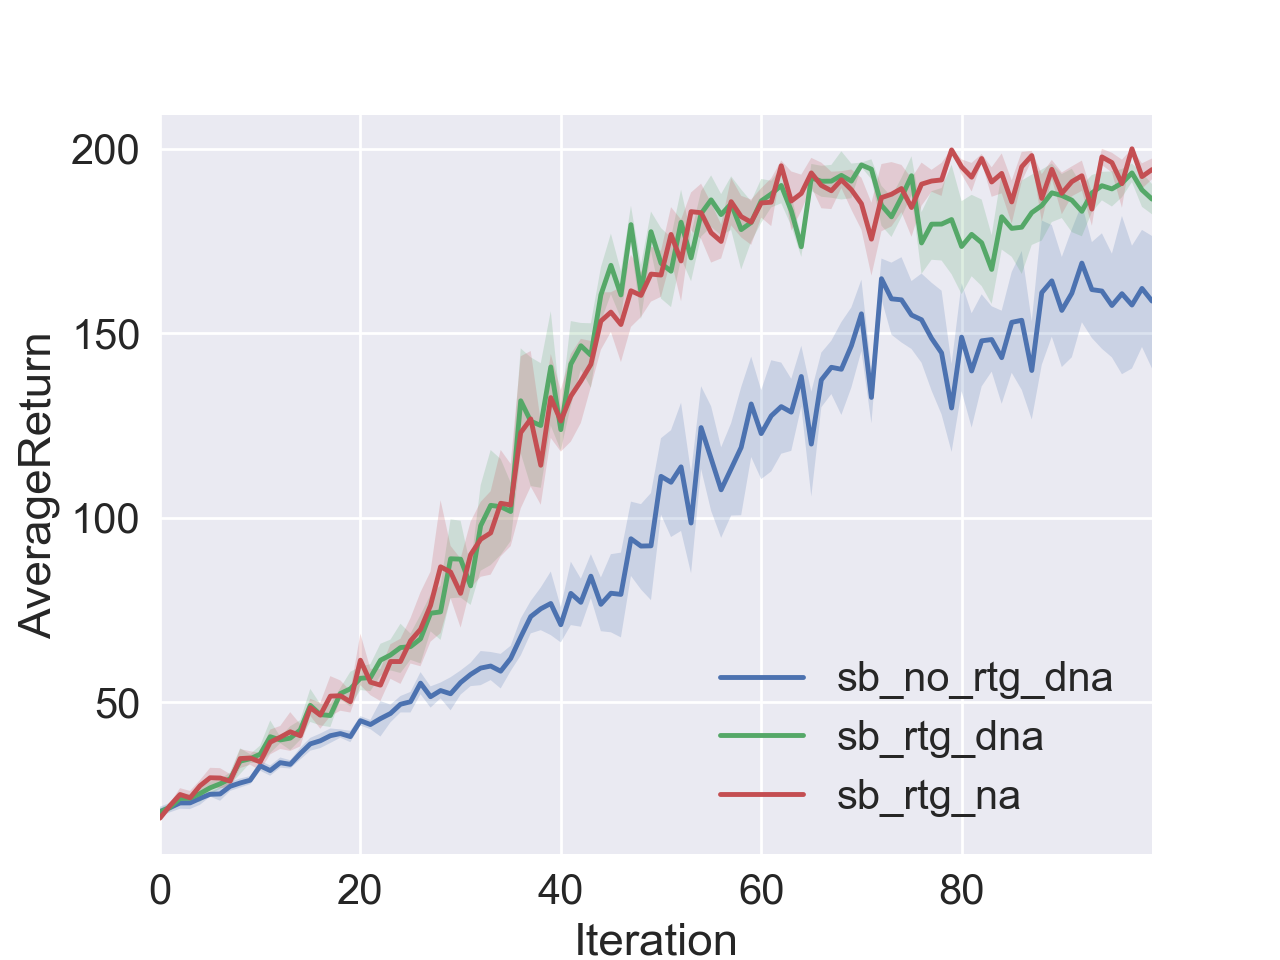
\includegraphics[width=\linewidth]{figures/4_2_1_sb.png}
  \captionof{figure}{learning curves for experiments using small batch size}
\end{minipage}%
\hfill
\begin{minipage}{.47\textwidth}
  \centering
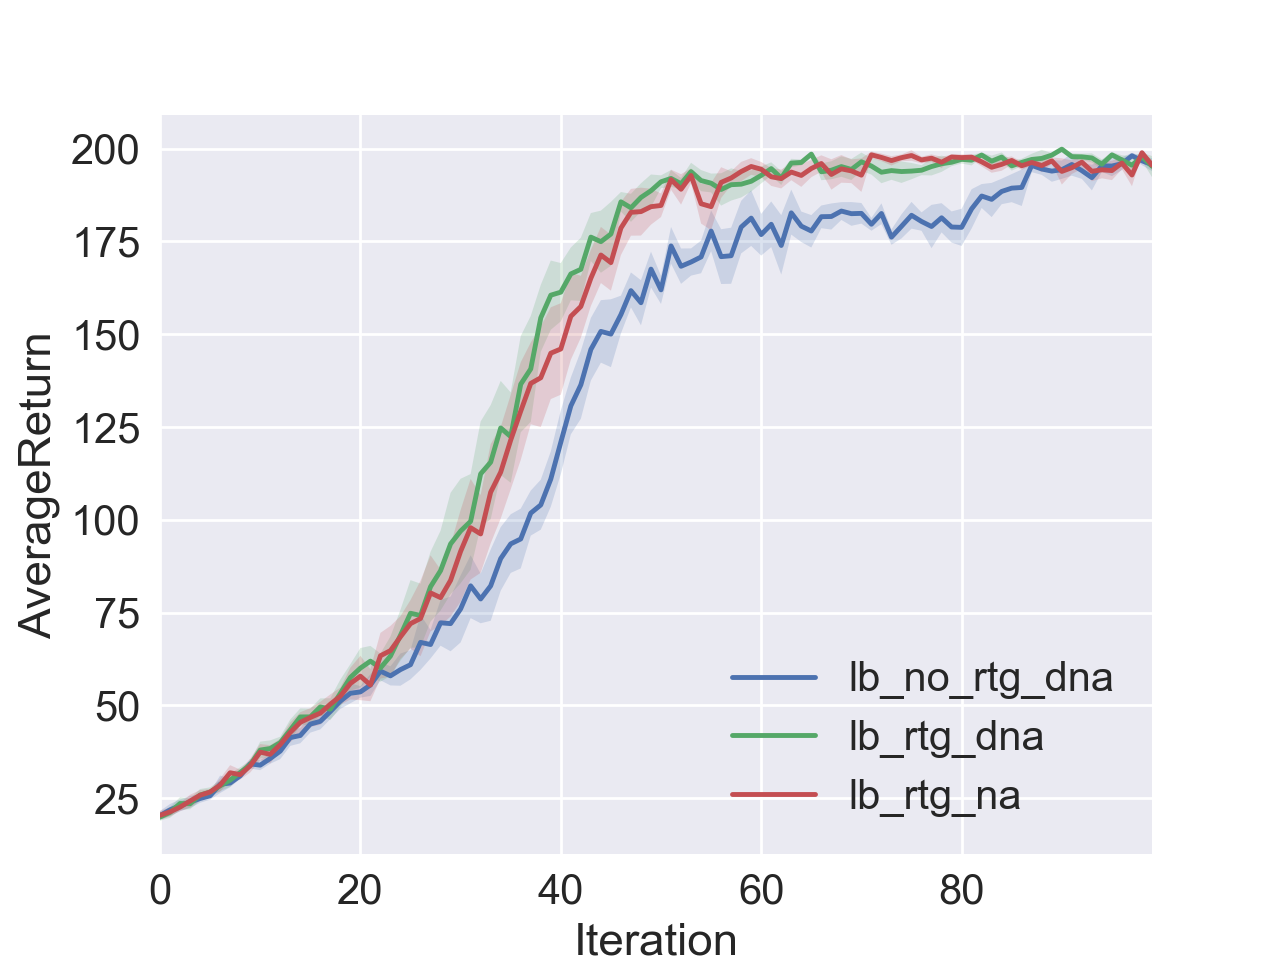
\includegraphics[width=\linewidth]{figures/4_2_1_lb.png}
\captionof{figure}{learning curves for experiments using large batch size}
\end{minipage}
\end{figure}

Based on the experiment results, we have the following observations:
\begin{enumerate}
\item Without advantage-centering (experiments with \textbf{dna}), the one using reward to go is better than the trajectory-centric one, for both small batch size and large batch size.
\item We only make advantage centering available when we use reward to go. From the learning curves, it's hard to say advantage centering helps.
\item By using reward to go, we expect to get a better performance from the theory as this does not change the expectation of policy gradient but reduces the variance of the gradient estimator. This matches our empirical results. Meanwhile, theoretically to perform advantage normalization should lower the variance of the gradient estimator and help boost the empirical performance, this is not observed in our empirical results. One possible explanation is that CartPole-v0 is an easy task with all the immediate rewards being constantly $1$ before the end of the task. For an environment with more complex reward function, the story may be different.
\item From figure $3$ to $5$ we can tell that a larger batch size in general help, but the improvement is limited after we use reward to go.
\end{enumerate}

\begin{figure}[H]
\centering
\begin{minipage}{.3\textwidth}
  \centering
  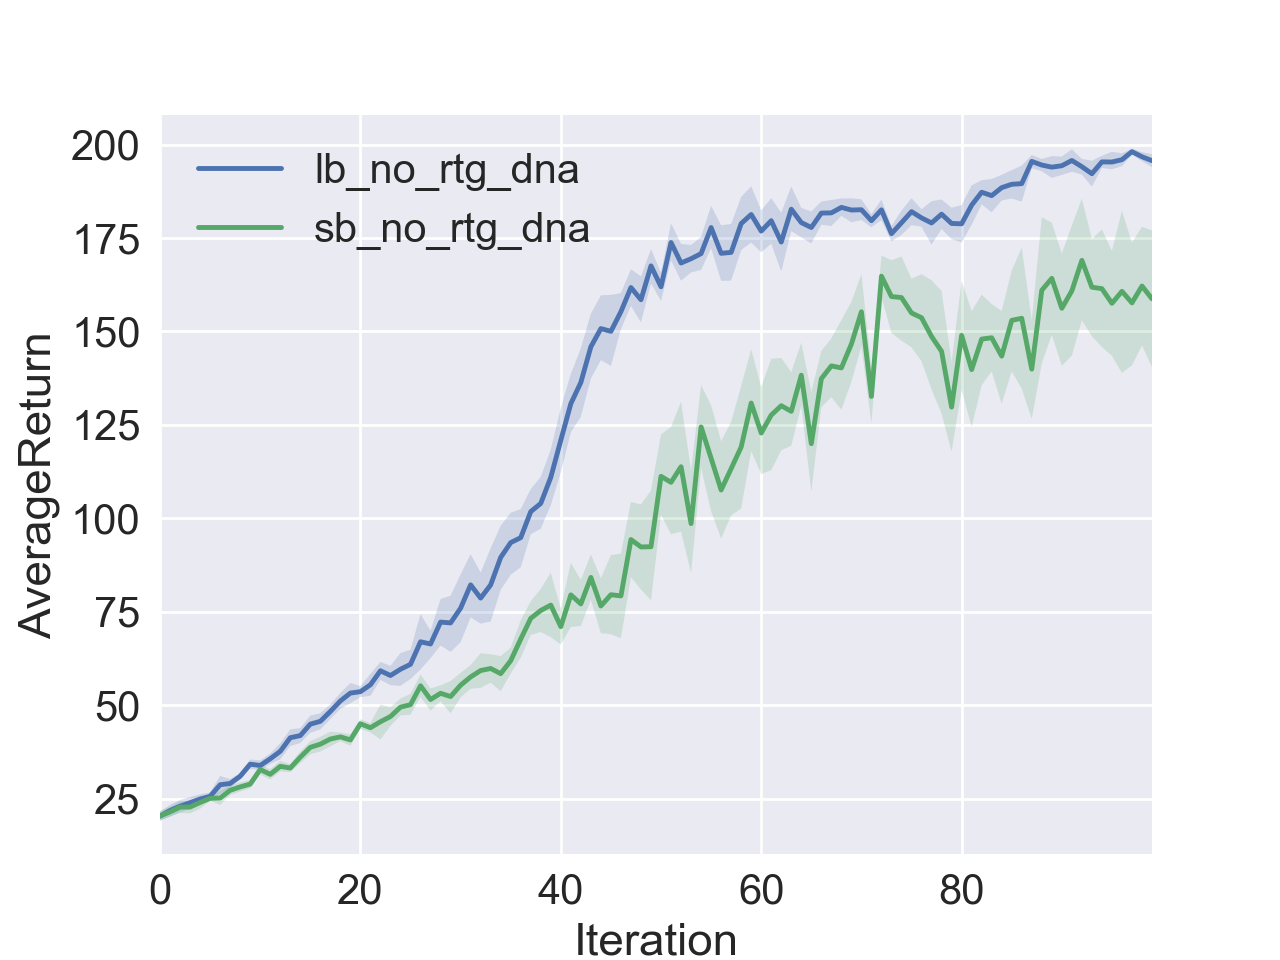
\includegraphics[width=\linewidth]{figures/4_2_1_no_rtg_dna.png}
  \captionof{figure}{learning curves for experiments using small batch size}
\end{minipage}%
\hfill
\begin{minipage}{.3\textwidth}
  \centering
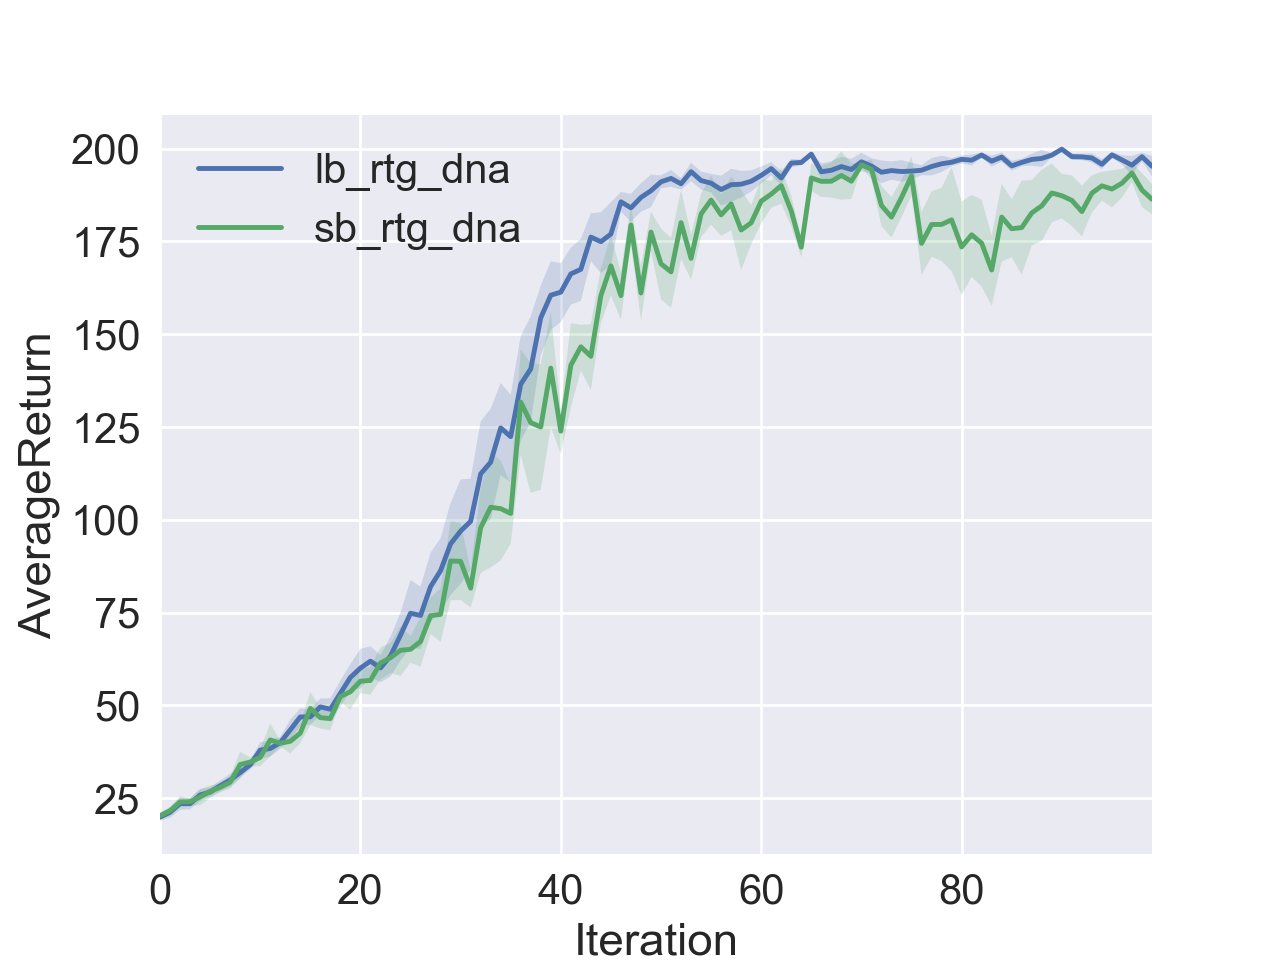
\includegraphics[width=\linewidth]{figures/4_2_1_rtg_dna.png}
\captionof{figure}{learning curves for experiments using large batch size}
\end{minipage}
\hfill
\begin{minipage}{.3\textwidth}
  \centering
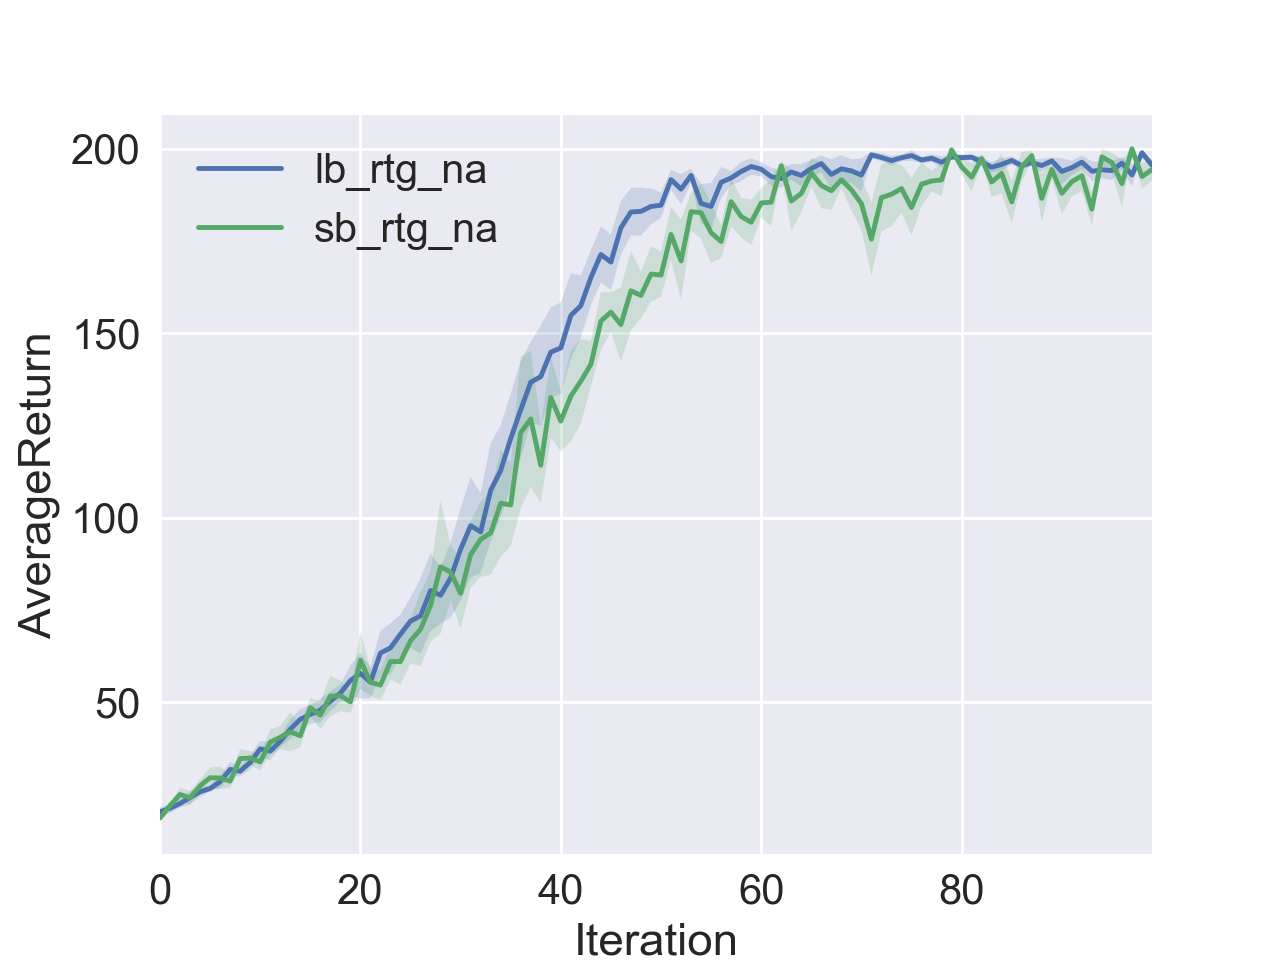
\includegraphics[width=\linewidth]{figures/4_2_1_rtg_na.png}
\captionof{figure}{learning curves for experiments using large batch size}
\end{minipage}
\end{figure}

\subsubsection*{2}

Using the following hyperparameters:
\begin{itemize}
\item \textbf{batch size}: 2000
\item \textbf{use reward to go}
\item \textbf{use advantage normalization}
\item \textbf{discount factor}: $1.0$ (no discount)
\item \textbf{number of random seeds}: $1$
\item \textbf{random seed}: $1$
\item \textbf{number of iterations}: $100$
\item \textbf{max path length}: $1000$, which is enforced by OpenAI's design of max number of timesteps allowed in an episode for InvertedPendulum-v1
\item \textbf{learning rate}: $0.005$
\item \textbf{optimization}: Adam with its default setting in PyTorch
\item \textbf{policy architecture}: see figure \ref{fig:arch}

\end{itemize}

\begin{figure}[H]
\centering
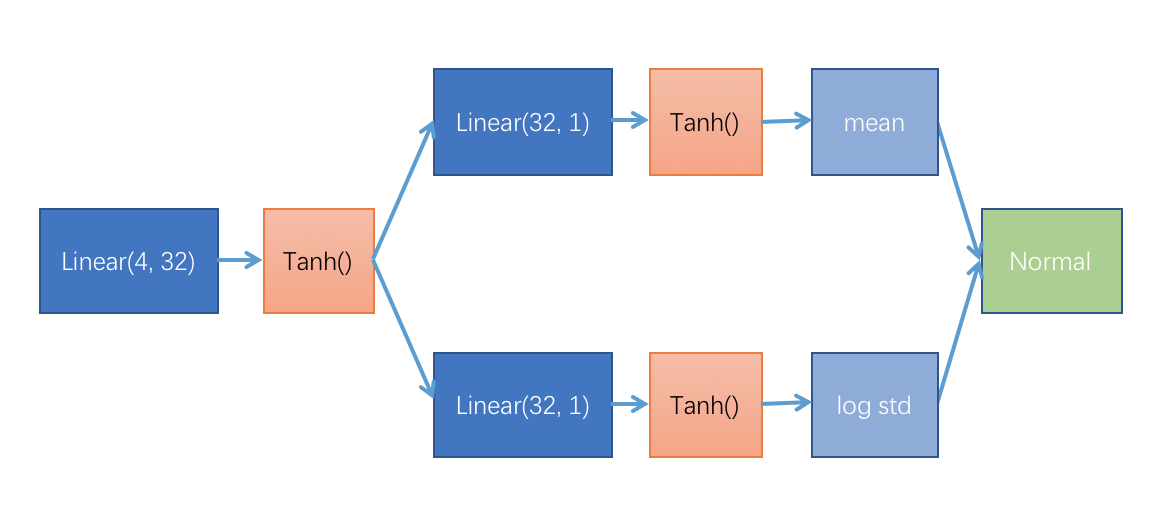
\includegraphics[width=0.75\linewidth]{figures/model_architecture_4_2_2.png}
\caption{model architecture for policy network in $4.2.2$}
\label{fig:arch}
\end{figure}

by running the following command line configuration \footnote{-tm is used to indicate whether we want to apply a tanh activation function for the mean of the Normal distribution and -ts is used to indicate whether we want to apply a tanh activation function for $\log{\text{std}}$ of the Normal distribution.},
\begin{lstlisting}[language=bash]
python train_pg.py InvertedPendulum-v1 -n 100 -b 2000 -l 1 -s 32 -e 1 -rtg 
    -lr 5e-3 -ts -tm --exp_name b2000_l1_s32
\end{lstlisting}
we obtain the learning curve in figure \ref{fig:lc}.

\begin{figure}[H]
\centering
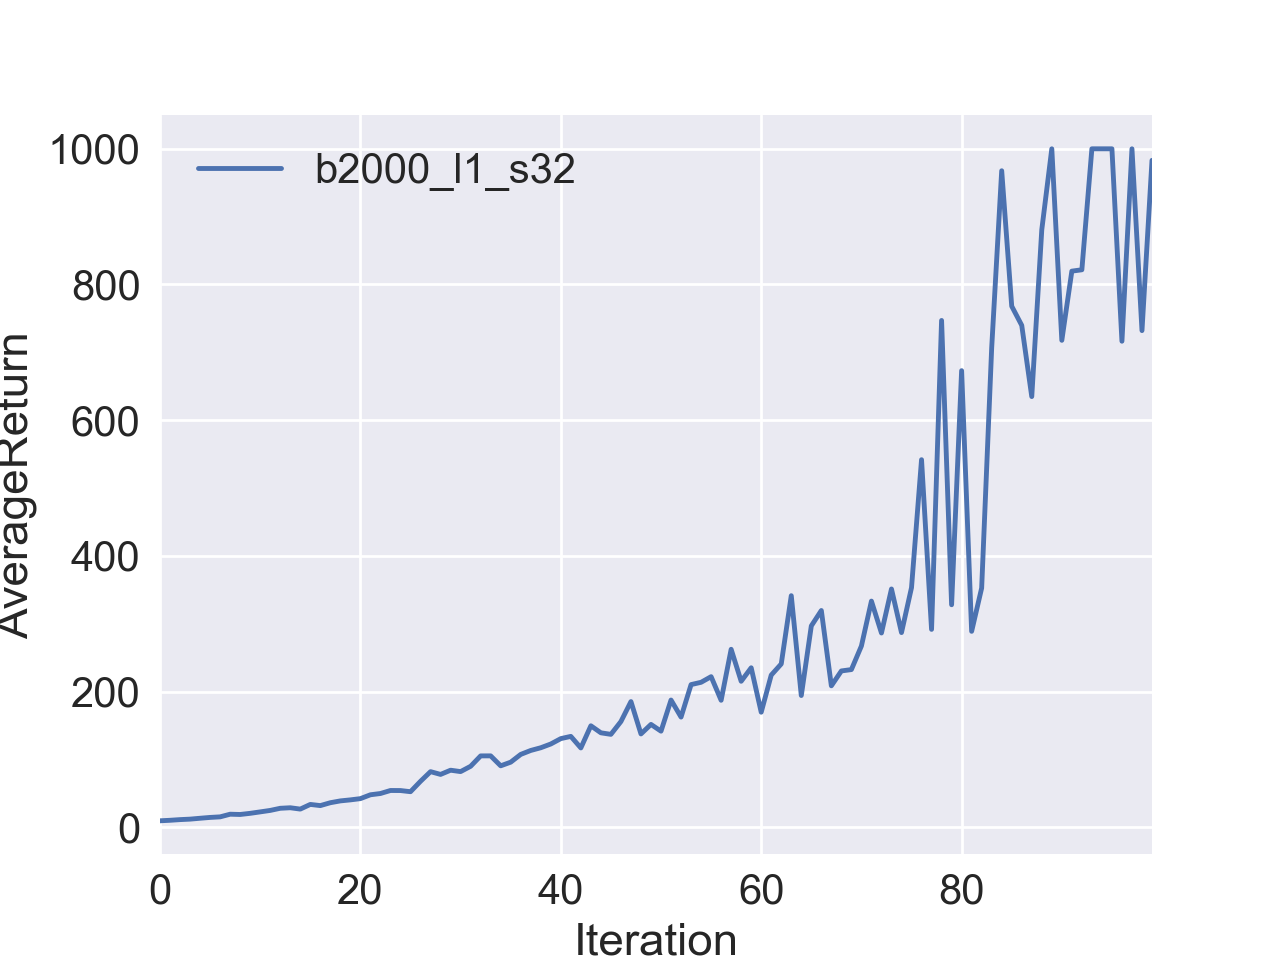
\includegraphics[width=0.4\linewidth]{figures/learning_curve_4_2_2.png}
\caption{learning curve for the experiment requires in 4.2.2}
\label{fig:lc}
\end{figure}

\section*{5 Implement  Neural Network Baselines}

For the objective of the baseline, we simply use mean squared error with the target being the reward to go for the on-policy experience, i.e.
\begin{equation}
\frac{1}{\sum_{i=1}^{N}T_{i}}\sum_{i=1}^{N}\sum_{t=1}^{T_{i}}\left|\left|\hat{V}_{\phi}^{\pi}(s_{i, t})-\sum_{t'=t}^{T_{i}}r(s_{i, t}, a_{i, t})\right|\right|^{2},
\end{equation}
where $N$ is the number of trajectories, $s_{i,t}, a_{i,t}$ is the $t$th state, action in trajectory $i$ and $T_{i}$ is the length of the $i$th trajectory.\\

We perform two experiments to compare the learning curve with both the neural network baseline function and advantage normalization to that without the neural network baseline function but with advantage normalization. We use the same hyperparameters as in the previous section except that the learning curve is now averaged over $10$ random seeds $(1, 11, 21, 31, 41, 51, 61, 71, 81, 91)$.\\

The difference between using baseline or not is so small that we cannot conclude here whether the use of baseline helps.\\

\begin{figure}[H]
\centering
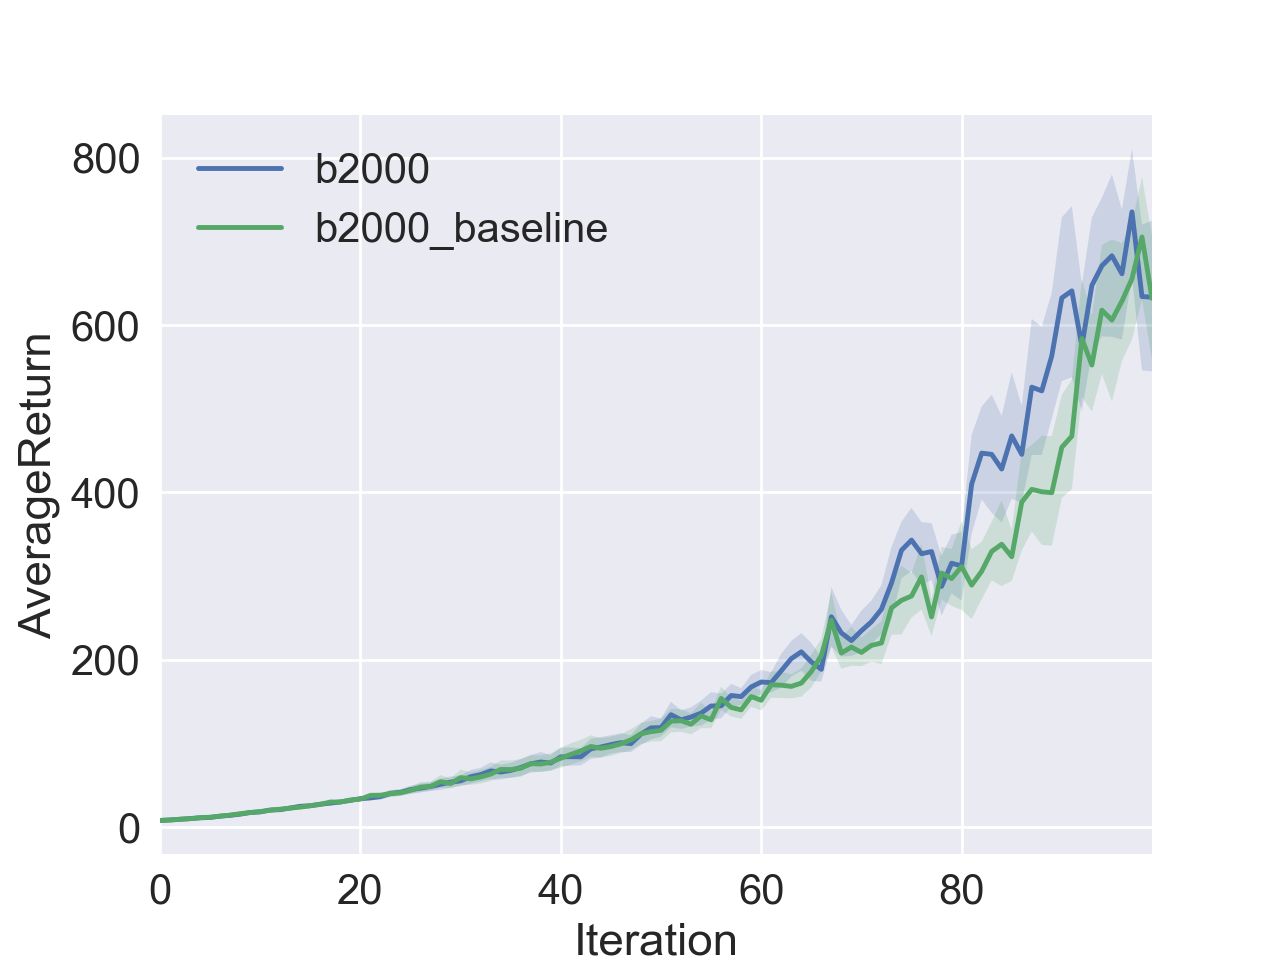
\includegraphics[width=0.4\linewidth]{figures/baseline.png}
\caption{b2000 refers to the learning curve without baseline while b2000$\rule{0.15cm}{0.15mm}$baseline refers to the one with baseline}
\end{figure}

It might be interesting to explore whether to set the target to be $n$-step bootstrapping, i.e., 
\begin{equation}
\sum_{\tau=1}^{n}r(s_{i, t+\tau-1}, a_{i, t+\tau-1}) + \hat{V}_{\phi}^{\pi}(s_{i, t+n}) \text{ for state }s_{i, t},
\end{equation}
in mean squared error would make a significant difference.

\section*{6 HalfCheetah}

We use the following hyperparameters and settings:
\begin{itemize}
\item \textbf{batch size}: $50000$
\item \textbf{use reward to go}
\item \textbf{use advantage normalization}
\item \textbf{use baseline}
\item \textbf{baseline objective}: same as the previous section 
\item \textbf{discount factor}: $0.9$
\item \textbf{number of random seeds}: $1$
\item \textbf{random seed}: $1$
\item \textbf{number of iterations}: $100$
\item \textbf{max path length}: $150$
\item \textbf{learning rate}: $0.025$
\item \textbf{optimization}: Adam with its default setting in PyTorch
\item \textbf{policy architecture}: see figure \ref{fig:6_policy} \footnote{Strictly speaking, we should use a multivariate normal distribution rather than a normal distribution which assumes that the covariance between any two distinct actions is $0$. However in practice this often make little difference.}
\item \textbf{critic (state value function estimator) architecture}:see figure \ref{fig:6_value}
\end{itemize}

\begin{figure}[H]
\centering
\begin{minipage}{.45\textwidth}
  \centering
  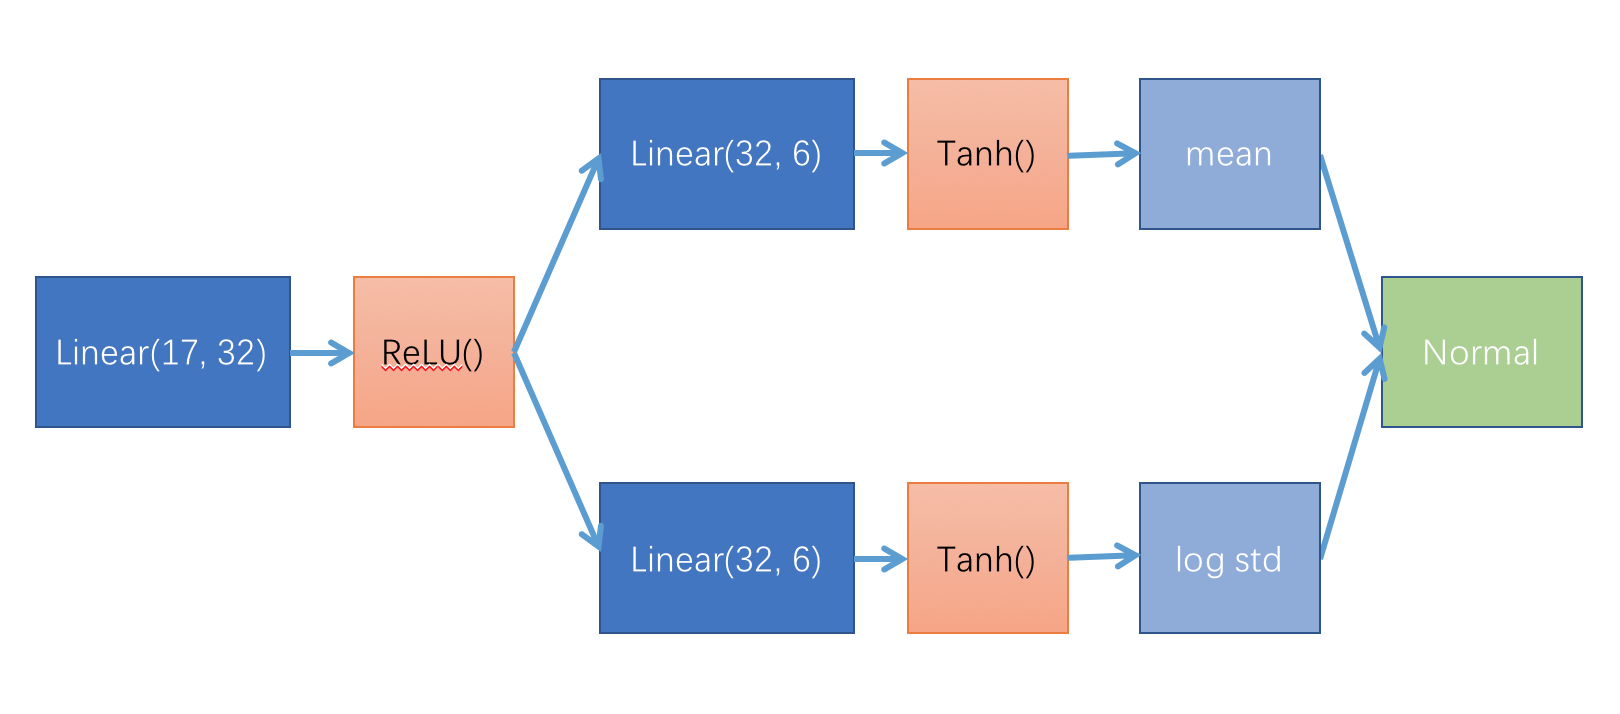
\includegraphics[width=\linewidth]{figures/6_policy.png}
  \captionof{figure}{policy network}
  \label{fig:6_policy}
\end{minipage}%
\hfill
\begin{minipage}{.45\textwidth}
  \centering
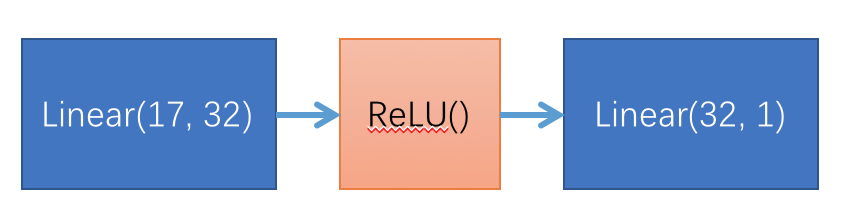
\includegraphics[width=\linewidth]{figures/6_value.png}
\captionof{figure}{value network}
\label{fig:6_value}
\end{minipage}
\end{figure}

, which corresponding to the command line configuration:
\begin{lstlisting}[language=bash]
python train_pg.py HalfCheetah-v1 -ep 150 --discount 0.9 -n 100 -b 50000 -l 1 
	-s 32 -e 1 -rtg -lr 0.025 -ts -tm -bl -ia relu 
    	--exp_name b50000_l1_s32_e1_rtg_ts_tm_bl_relu
\end{lstlisting}

We obtain the learning curve in figure \ref{fig:HalfCheetah} after performing the experiment.

\begin{figure}[H]
\centering
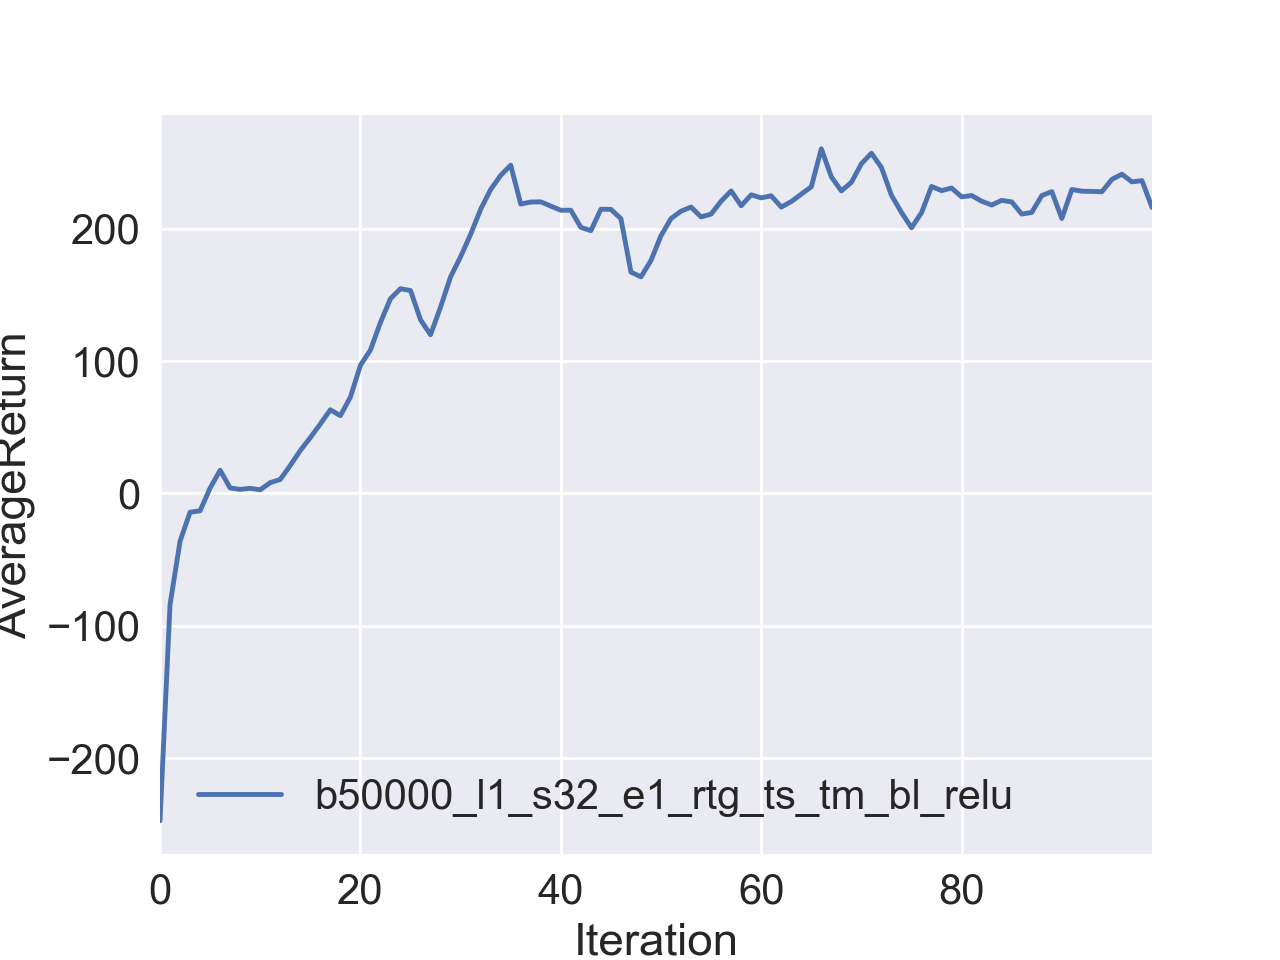
\includegraphics[width=0.4\linewidth]{figures/HalfCheetah.png}
\caption{The average return fluctuates around 220.}
\label{fig:HalfCheetah}
\end{figure}

\end{document}
